\begin{figure}[h]
    \centering
    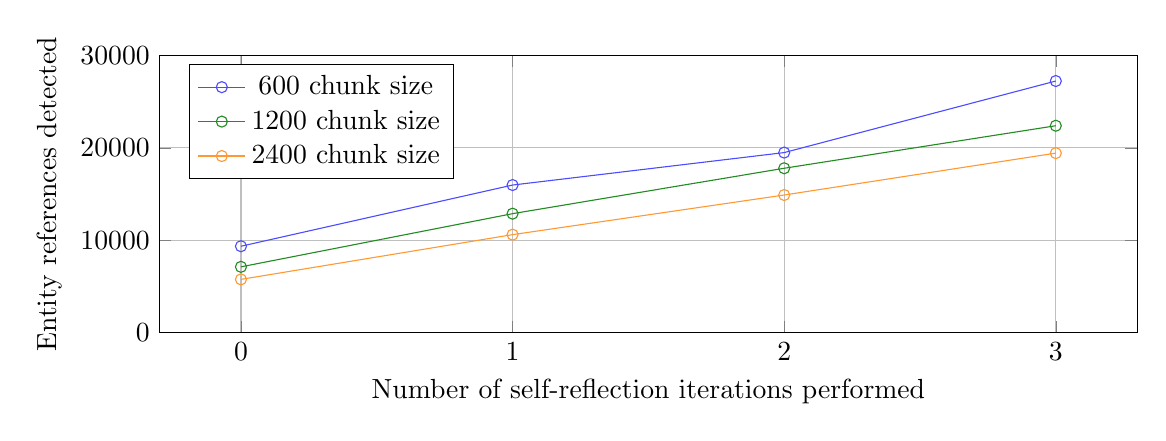
\begin{tikzpicture}
        \begin{axis}[
            xlabel={Number of self-reflection iterations performed},
            ylabel={Entity references detected},
            ytick={0,10000,20000,30000},
            yticklabels={0,10000,20000,30000},
            ymin=0,
            ymax=30000,
            xtick={0,1,2,3},
            legend pos=north west,
            grid=both,
            width=14cm,
            height=5.1cm,
            scaled y ticks=false
        ]
        
        \addplot[mark=o, blue!70] coordinates {
            (0, 9348)
            (1, 15976)
            (2, 19491)
            (3, 27240)
        };
        \addlegendentry{600 chunk size};

        \addplot[mark=o, ForestGreen] coordinates {
            (0, 7119)
            (1, 12877)
            (2, 17794)
            (3, 22399)
        };
        \addlegendentry{1200 chunk size};

        \addplot[mark=o, orange!80] coordinates {
            (0, 5761)
            (1, 10606)
            (2, 14897)
            (3, 19433)
        };
        \addlegendentry{2400 chunk size};
        \end{axis}

    \end{tikzpicture}
    \caption{How the entity references detected in the HotPotQA dataset~\citep{yang2018hotpotqa}}  varies with chunk size and self-reflection iterations for our generic entity extraction prompt with \texttt{gpt-4-turbo}.
    \label{fig:chunkentities}
\end{figure}